%% !TeX program = lualatex

%\listfiles	
% **************************
% STOP - Bitte zuerst lesen, bevor Sie weitermachen
%
% Einige Dinge müssen Sie an Ihre Bedürfnisse (und die Vorgaben Ihres
% Betreuers anpassen. Editieren Sie dazu die Datei docinfo.tex).
%
% 1. Sprache
% Das Template unterstützt Deutsch und Englisch, Standard ist Deutsch.
% Wenn Sie Englisch verwenden wollen, ändern Sie bitte direkt am Anfang
% dieser Datei den Eintrag
%    \newcommand{\hsmasprache}{de}
% auf
%    \newcommand{\hsmasprache}{en}
%
% 2. Form der Abgabe
% Das Template unterstützt sowohl eine digitale Abgabe, als auch eine Abgabe
% auf Papier. Bei einer Papierabgabe wird ein doppelseitiger Druck vorbereitet
% und der Titel wird so platziert, dass er in das Fenster des offiziellen
% Umschlages der Technischen Hochschule passt.
% Bei einer digitalen Abgabe (als PDF) wird der Titel zentriert und als
% Format wird einseitig gewählt. Außerdem wird die Datei unterschrift.png
% auf dem Blatt mit der Erklärung zur Eigenständigkeit eingebunden.
%
% 3. Zitierstil
% Abhängig von dem gewünschten Zitierstil passen Sie bitte in
% hma.cls die Einstellungen bei \RequirePackage[backend=biber...
% an. Wie ist dort genau erklärt.
% Achtung: Wenn Sie als Zitierstil Fußnoten wählen bzw. generell
% -------  mit Fußnoten arbeiten, dann beachten Sie bitte, dass
%          Fußnoten in Bildunterschriften und Tabellenüberschriften
%          nicht funktionieren.
%          Siehe hierzu https://texfaq.org/FAQ-ftncapt
%          und https://texfaq.org/FAQ-footintab
%          Sinnvollerweise verzichten Sie auf Fußnoten an diesen
%          Stellen und fügen Quellen einfach per \parancite ein.
%
% 4. Doppelseitiger oder einseitiger Druck
% Das Template bestimmt, ob einseitig oder doppelseitig gedruckt wird
% anhand der Abgabeform (papier / digital). Wollen sie dies übersteuern,
% müssen Sie in der Datei preambel.tex folgende Zeile
% \KOMAoptions{twoside=true} für doppelsetigen Druck
% \KOMAoptions{twoside=false} für einsetigen Druck
% direkt vor \usepackage{xcolor} einsetzen. Prinzipiell sollten Sie aber
% das vorgeschlagene Format einfach so lassen.
%
% 5. Unnötige Teile entfernen
% Entfernen Sie die Teile, die Sie nicht brauchen, z.B. Anhänge
%
% 6. Silbentrennung
% LaTeX führt eine automatische Silbentrennung durch. Allerdings
% werden Wörter, die bereits einen Bindestrich enthalten nicht
% getrennt, z.B. Datenschutz-Grundverordnung. Wenn Sie Ihren Text auf
% Deutsch schreiben, können Sie dann alternativ "= für den Bindestrich
% im Wort verwenden, z.B. Datenschutz"=Grundverordnung, damit LaTeX
% weiterhin richtig trennt.
% Ist die Silbentrennung aus einem anderen Grund nicht erfolgt, sodass
% das Wort über den rechten Rand hinaussteht oder wenn Sie eine weitere
% Trennstelle wollen, können Sie LaTeX helfen, indem Sie weitere
% Trennstellen angeben. Dies geschieht durch "- als Zeichen, z.B.
% Staats"-vertrag.
%
% 7. Nummerierung der Fußnoten
% LaTeX beginnt die Nummerierung der Fußnoten in jedem Kapitel wieder
% bei 1. In diesem Template wird die fortlaufende Nummerierung der Fußnoten 
% über die gesamte Arbeit umgesetzt.  
%
% 8. Unterschrift
% Bei einer Abgabe auf Papier unterschreiben Sie die Arbeit eigenhändig.
% Geben Sie allerdings digital ab, sollten Sie die Datei unterschrift.png in dem 
% Ordner /bilder durch einen Scan Ihrer eigenen Unteschrift ersetzen - andernfalls
% unterschreiben Sie als Max Mustermann ;-)
% *******************************************************************


% Dokumenteneinstellungen und Infos importieren
% -------------------------------------------------------
% Informationen und Einstellungen für Ihre Abschlussarbeit
%

% Sprache für das Dokument festlegen
\newcommand{\hsmasprache}{de} %de für Deutsch oder en für Englisch


% Abgabeform festlegen
% Bei einer digitalen Abgabe, wird das Dokument einseitig erzeugt und der Titel wird
% zentriert.
\newcommand{\hsmaabgabe}{digital} % Abgabe erfolgt für Fakultät I digital. Optionen hier sind für anderen Fakultäten: "papier" oder "digital".


% Flags für Veröffentlichung, Sperrvermerk
\newcommand{\hsmapublizieren}{opensource}   
% Wird einer Veröffentlichung zugestimmt?
% Optionen: 
% opensource = Druck der CC Lizenz mit By SA (Standard)
% hs = Veröffentlichung an der Technischen Hochschule und auf Hochschulservern
% stud = kein opensource und keine veröffentlichung auf den Hochschulservern
% vertraulich = Arbeit darf nicht veröffentlicht werden und erhält einen Sperrvermerk (Nur nach Absprache mit Betreuer setzen!)


\newcommand{\genderhinweis}{gender}     % Soll der Gender-Hinweis angezeigt werden? ja=gender, nein = nogender; Genderhinweis wird nur in deutscher Sprache angezeigt!


\newcommand{\hsmaquellcode}{sourcecode} % Verwenden Sie Quellcode in Ihrer Arbeit? ja=sourcecode, nein= nosourcecode

\newcommand{\hsmasymbole}{symbole} % Verwenden Sie viele Symbole in Ihrer Arbeit, welche in einem Symbolverzeichnis aufgeführt werden sollen? ja=symbole, nein= nosymbole


\newcommand{\hsmaglossar}{glossar} % Verwenden Sie Begriffserklärungen nicht Abkürzungen in Ihrer Arbeit? ja=glossar, nein= noglossar

\newcommand{\hsmatc}{tc} % Verwenden der Änderungsmarkierung. Änderungsmarkierung aktiv und eine Liste der Änderungen wird angezeigt = tc, Keine Änderungsmarkierung und keine Ausgabe der Änderungen = notc




% Titel der Arbeit auf Deutsch
\newcommand{\hsmatitelde}{Eindeutige Produktzuordnung zur Schwachstellenanalyse: Modellierung von Produkten zur Abbildung mit heterogenenen Schwachstellendatenbanken}

% Titel der Arbeit auf Englisch
\newcommand{\hsmatitelen}{AUTO-TRANSLATED: Unambiguous Product Mapping for Vulnerability Analysis: Modeling of Products for Integration with Heterogeneous Vulnerability Databases}

% Weitere Informationen zur Arbeit
\newcommand{\hsmaort}{Mannheim}        % Ort
\newcommand{\hsmaautorvname}{Yan}      % Vorname(n)
\newcommand{\hsmaautornname}{Wittmann} % Nachname(n)
\newcommand{\hsmaabgabedatum}{2025-07-21} % Datum der Abgabe in dem Format JJJJ-MM-TT

\newcommand{\hsmafirma}{\{metæffekt\} GmbH} % Firma bei der die Arbeit durchgeführt wurde
\newcommand{\hsmabetreuer}{Prof. Thomas Smits, Technische Hochschule Mannheim} % Betreuer an der Hochschule
\newcommand{\hsmazweitkorrektor}{Karsten Klein, \{metæffekt\} GmbH}   % Betreuer im Unternehmen oder Zweitkorrektor

\newcommand{\hsmafakultaet}{I}    % I für Informatik oder E, S, B, D, M, N, W, V
\newcommand{\hsmastudiengang}{IB} % IB IMB UIB CSB IM MTB (weitere siehe titleblatt.tex)


% Preambel importieren
% Dokumententyp, benutzte Pakete und deren Einstellungen
\documentclass[	\hsmasprache,%
				\hsmaabgabe,%
				\hsmapublizieren,%
				\genderhinweis,
				\hsmaquellcode,
				\hsmasymbole,
				\hsmaglossar,
				\hsmatc]{HMA}

% Wo sind die Bilder?
\graphicspath{{bilder/}}


% Wo liegt Sourcecode?
\newcommand{\srcloc}{src/}


% Checklisten mit zwei Ebenen
\newlist{checklist}{itemize}{2}
\setlist[checklist]{label=$\square$}



% Befehl zum Erstellen eigener Makros. In diesem Fall ist es ein Makro für das Einbinden von Bildern. Das label (für \ref) ist dann der Name der Bilddatei
\newcommand{\bild}[3]{
	\begin{figure}[ht]
		\centering
		\includegraphics[width=#2]{#1}
		\caption{#3}
		\label{#1}
\end{figure}}




							


\newcommand{\snowcard}[9]{
	\begin{table}[ht!]
		\caption{\hsmasnowcardanforderung\ #1 -- #4}\label{#1}
		\renewcommand{\arraystretch}{1.2}
		\centering
		\sffamily
		\begin{footnotesize}

			\begin{tabularx}{\linewidth}{sssssl}
				\toprule
				\textbf{\hsmasnowcardno} & #1 & \textbf{\hsmasnowcardart} & #2 & \textbf{\hsmasnowcardprio} & #3 \\
				\midrule
				\multicolumn{2}{l}{\textbf{\hsmasnowcardtitel}} & \multicolumn{4}{l}{\parbox[t]{11.8cm}{#4}} \\
				\ifx&#5&%
				\else
				\multicolumn{2}{l}{\textbf{\hsmasnowcardherkunft}} & \multicolumn{4}{l}{\parbox[t]{11.8cm}{#5}} \\
				\fi
				\ifx&#6&%
				\else
				\multicolumn{2}{l}{\textbf{\hsmasnowcardkonflikt}} & \multicolumn{4}{l}{\parbox[t]{11.8cm}{#6}} \\
				\fi
				\addlinespace
				\multicolumn{6}{l}{\textbf{\hsmasnowcardbeschreibung}} \\
				\multicolumn{6}{l}{\parbox[t]{13.5cm}{#7\strut}} \\
				\ifx&#8&%
				\else
				\addlinespace
				\multicolumn{6}{l}{\textbf{\hsmasnowcardfitkriterium}} \\
				\multicolumn{6}{l}{\parbox[t]{13.5cm}{#8\strut}} \\
				\fi
				\ifx&#9&%

				\else
				\addlinespace
				\multicolumn{6}{l}{\textbf{\hsmasnowcardmaterial}} \\
				\multicolumn{6}{l}{\parbox[t]{13.5cm}{#9\strut}} \\
				\fi
				\bottomrule
			\end{tabularx}
		\end{footnotesize}
	\end{table}
}



% Quality Attribute Scenario
\newcommand{\qas}[9]{
	\begin{table}[ht!]
		\caption{\hsmaqasanforderung\ #1 -- #3}\label{#1}
		\renewcommand{\arraystretch}{1.2}
		\centering
		\sffamily
		\begin{footnotesize}

			\begin{tabularx}{\linewidth}{sssssl}
				\toprule
				\textbf{\hsmaqasno} & #1 & \textbf{\hsmaqasart} & QAS & \textbf{\hsmaqasprio} & #2 \\
				\midrule
				\multicolumn{2}{l}{\textbf{\hsmaqastitel}} & \multicolumn{4}{l}{\parbox[t]{11.8cm}{#3}} \\
				\multicolumn{2}{l}{\textbf{\hsmaqasquelle}} & \multicolumn{4}{l}{\parbox[t]{11.8cm}{#4}} \\
				\multicolumn{2}{l}{\textbf{\hsmaqasstimulus}} & \multicolumn{4}{l}{\parbox[t]{11.8cm}{#5}} \\
				\multicolumn{2}{l}{\textbf{\hsmaqasartefakt}} & \multicolumn{4}{l}{\parbox[t]{11.8cm}{#6}} \\
				\addlinespace
				\multicolumn{6}{l}{\textbf{\hsmaqasumgebung}} \\
				\multicolumn{6}{l}{\parbox[t]{13.5cm}{#7\strut}} \\
				\addlinespace
				\multicolumn{6}{l}{\textbf{\hsmaqasantwort}} \\
				\multicolumn{6}{l}{\parbox[t]{13.5cm}{#8\strut}} \\
				\addlinespace
				\multicolumn{6}{l}{\textbf{\hsmaqasmass}} \\
				\multicolumn{6}{l}{\parbox[t]{13.5cm}{#9\strut}} \\
				\bottomrule
			\end{tabularx}
		\end{footnotesize}
	\end{table}
}




%Abstrakt Ihrer Abschlussarbeit
% -------------------------------------------------------
% Abstrakt / Abstract
% Achtung: Wenn Sie im Abstrakt Anführungszeichen verwenden wollen, dann benutzen Sie
%          nicht "` und "', sondern \enquote{}. "` und "' werden nicht richtig
%          erkannt.

% Kurze (maximal halbseitige) Beschreibung, worum es in der Arbeit geht auf Deutsch
\newcommand{\hsmaabstractde}{
    Um Softwareartefakte verschiedenen Produktrepräsentationen wie CPE, PURL oder Produktkennungen von Microsoft zuordnen zu können, wurde in dieser Arbeit ein neues System für die Modellierung von Beziehungen zwischen Produkten für das Schwachstellen\-management-System der \metaeffektsp GmbH entwickelt.
    Ausgangspunkt ist eine Analyse der Schwächen des bisherigen YAML-basierten Formats, darunter die Übergeneralisierung von Regeln zur Auswahl von Artefakten, uneinheitliche Typangaben und eingeschränkt nachvollziehbare Entscheidungen.
    Als Lösung wurde ein graphenbasiertes Modell entworfen, in dem Produkte und ihre verschiedenen Darstellungen als Knoten erfasst und ihre Beziehungen durch Kanten beschrieben werden.
    Dieses Modell wurde in Java zur Demonstration der Funktionsfähigkeit umgesetzt und nutzt SQLite zur Speicherung der Daten.
    Durch eine Analyse der möglichen Datenquellen werden im neuen System typische Merkmale der Daten genutzt, um typspezifische Attribute für genauere und bewusstere Zuordnungen explizit bereitzustellen.
    Manuelle Anpassungen bleiben weiterhin über ein manuelles Modifikationsformat möglich.
    Zudem wird die automatische Generierung von Inahlten aus öffentlichen Datenanteilen und innere Konsistenzprüfung behandelt.
}

% Kurze (maximal halbseitige) Beschreibung, worum es in der Arbeit geht auf Englisch
\newcommand{\hsmaabstracten}{
    In order to reliably assign software artefacts to various product representations such as CPEs, PURLs, or Microsoft product identifiers, this thesis presents the development of a new system for modeling relationships between products for the vulnerability management system of \metaeffektsp GmbH.
    The work begins with an analysis of the limitations of the existing YAML-based correlation solution, which include overly broad selection rules, inconsistent type matching, and limited traceability of decision logic.
    As a solution, a graph-based model was designed, in which products and their representations are expressed as nodes, and their relationships are described through typed edges.
    This model was implemented in Java to demonstrate its feasibility and uses SQLite for data storage.
    Based on an analysis of common input sources, the new system identifies characteristic patterns to extract type-specific attributes, enabling more accurate and deliberate correlations.
    Manual adjustments remain possible by applying a dedicated modification format.
    The system also addresses the automated generation of graph contents from public data sources and ensures internal consistency through validation mechanisms
}



% Literatur-Datenbank
\addbibresource{literatur.bib}   % BibLaTeX-Datei mit Literaturquellen einbinden


% Anfang des Dokuments
\begin{document}	


%Laden der Dateien mit Abkürzungen, Begriffserklärungen (Glossar), Symbole
\newacronym{oss}{OSS}{Open Source Software}
\newacronym{cra}{CRA}{Cyber Resilliance Act}
\newacronym{cve}{CVE}{Common Vulnerabilities and Exposures}
\newacronym{cpe}{CPE}{Common Product Enumeration}
\newacronym{osv}{OSV}{Open Source Vulnerabilities}
\newacronym{msrc}{MSRC}{Microsoft Security Responce Center}
\newacronym{nist}{NIST}{National Institute of Standards and Technology}
\newacronym{vms}{VMS}{Vulnerability Management System}
\newacronym{vdb}{VDB}{Vulnerability Database}
\newacronym{nvd}{NVD}{National Vulnerability Database}
\newacronym{purl}{PURL}{Package URL}
\newacronym{cwe}{CWE}{Common Weakness Enumeration}
\newacronym{ciavuln}{CIA}{Confidentiality, Integrity, Availability}
\newacronym{api}{API}{Application Programming Interface}
\newacronym{cisa}{CISA}{Cybersecurity and Infrastructure Security Agency}
\newacronym[
  plural=CNAs,
  firstplural=CVE Numbering Authorities (CNAs)
]{cna}{CNA}{CVE Numbering Authority}
\newacronym{sbom}{SBOM}{Software Bill of Materials}
\newacronym{spdx}{SPDX}{System Package Data Exchange}
\newacronym{swid}{SWID}{Software Identification Tags}
\newacronym{cmu}{CMU}{Carnegie Mellon University}
\newacronym{scap}{SCAP}{Security Content Automation Protocol}
\newacronym{wfn}{WFN}{Well-Formed CPE Name}
\newacronym{yaml}{YAML}{Yet Another Markup Language}
\newacronym{csv}{CSV}{Comma Separated Value}
\newacronym{ide}{IDE}{Integrated Development Environment}
\newacronym{eol}{EOL}{End of Life (endoflife.date)}
\newacronym{bsi}{BSI}{Bundesamts für Sicherheit in der Informationstechnik}
\newacronym{ai-rnn}{RNN}{rekurrentes neuronales Netzwerk}

% Glossareinträge
\newglossaryentry{glos:amplification}{name={Amplification}, description={describes the disproportionate increase of a response packet compart to the initial request packet.}}

% Verzeichnis von Symbolen und Einheiten
\newglossaryentry{symb:Pi}{name=\ensuremath{\pi},
	description={Geometrical value},
	unit={},
	type=symbolslist}

\newglossaryentry{symb:energyconsump}{name=\ensuremath{P},
	description={Energy consumption},
	unit={\si{kW}},
	type=symbolslist}
	
	
\pagestyle{headings}
\tableofcontents


\mainmatter

%% Ihre Inhaltsdateien werden an dieser Stelle in das Dokument eingefügt
\chapter{Einleitung}\label{ch:einleitung}


\section{Hintergrund und Motivation}\label{sec:hintergrund-motivation}

Moderne Software wird zunehmend aus einer Vielzahl kleinerer Bestandteile zusammengesetzt, was die Art und Weise, wie Software entwickelt, verteilt und betrieben wird, grundlegend verändert hat.
Ein großer Anteil dieser Komponenten basiert auf \acrfull{oss} und dient damit als Grundlage digitaler Infrastrukturen in nahezu allen Branchen:
Laut dem Open Source Monitor des Bitkom e.V.\ setzen 69\% der deutschen Unternehmen \acrshort{oss} in ihren Lösungen ein\ \autocite{OpenSourceMonitorWintergerst}.

Mit der wachsenden Abhängigkeit von \acrshort{oss} steigt jedoch auch die Verantwortung für deren sichere und nachvollziehbare Verwendung.
In dem bereits verabschiedeten \acrfull{cra} der Europäischen Union geht es um die Cybersicherheit von Produkten mit digitalen Elementen und berücksichtigt dabei auch \acrshort{oss}-Komponenten.
Ab dem 11.\ Juni 2026 sind Unternehmen verpflichtet, bekannte Schwachstellen in ihrer Software-Lösung und den verwendeten Komponenten zu identifizieren und Sicherheitsvorfälle zu dokumentieren.
Spätestens ab dem 11.\ Dezember 2027 sind alle Vorgaben des \acrshort{cra} verbindlich.
Eine aktiv ausgenutzte Schwachstelle ist nach dem \acrshort{cra} ein meldepflichtiger Sicherheitsvorfall und muss innerhalb von 72 Stunden an die zuständigen Behörden gemeldet werden\ \autocite{eu2024cra}.

Eine der am weitesten verbreiteten Quellen für Schwachstelleninformationen ist das \acrfullr{cve}-System, das als Bestandteil der \acrfull{nvd} des \acrfull{nist}\footnote{\url{https://nvd.nist.gov/vuln}} mit derzeit fast 300.000 Einträgen die umfangreichste öffentlich zugängliche Schwachstellendatenbank darstellt\ \autocite{nvd12mai2025dashboard}.
Diese große Anzahl an erfassten Schwachstellen und der kontinuierliche Zuwachs machen es in Kombination mit den kurzen Meldefristen des \acrshort{cra} unmöglich, den Prozess der Schwachstellensuche rein manuell abzubilden.
Für 65\% der Unternehmen ist eine manuelle Überwachung dieser Datenmengen durch den zeitlichen Aufwand und das Risiko eines menschlichen Fehlers unmöglich\ \autocite{OpenSourceMonitorWintergerst}, weshalb sie automatisierte \acrfull{vms} einsetzen.

Moderne und automatisierte \acrshort{vms} verarbeiten die erfassten Softwareinventare typischerweise in mehreren Schritten, um den firmeneigenen Softwarekatalog mit relevanten Schwachstelleninformationen aus verknüpften \acrfullpl{vdb} abzugleichen:
die Identifikation der eingesetzten Komponenten, die Erkennung potenzieller Schwachstellen, eine regelbasierte Bewertung der Ergebnisse und die Erzeugung von Ergebnisberichten\ \autocite{Idrissi_Sebai_Faroukhi_Mahouachi_2024}.

Die Zuordnung der eigenen Komponenten zu den Produktbezeichnern der jeweils abzugleichenden \acrshort{vdb} ist als erster Schritt bereits einer der herausforderndsten.
Die \acrshort{nvd} etwa stellt mit dem \acrfull{cpe}-System ein Schema zur Verfügung, um Softwareprodukte zu identifizieren und zu \acrshort{cve} zuzuordnen\ \autocite{Cheikes_Waltermire_Scarfone_2011}.
In der Praxis ist die korrekte Abbildung der eingesetzen Komponenten auf \acrshort{cpe}-Einträge jedoch mit Schwierigkeiten verbunden:
uneinheitliche Benennungen, Doppelungen, Rechtschreibfehler und mehr führen zu Fehlidentifikationen und unvollständigen Ergebnissen im darauf folgenden Schwachstellen-Scan\ \autocite{Sanguino_Uetz_2017}.
Dies macht es unmöglich, sich ausschließlich auf die Ergebnisse dieser automatischen Scans zu verlassen und erfordert eine manuelle Kontrolle der Ergebnisse, insbesondere der erschlossenen Komponenten-Abbildungen\ \autocite{Sanguino_Uetz_2017}.

Das Problem beschränkt sich jedoch nicht auf die \acrshort{nvd} mit ihren \acrshort{cpe}, auch Produktbezeichner aus anderen Quellen wie die \acrfull{osv}-Datenbank\footnote{\url{https://osv.dev}}, den \acrfull{msrc} Update Guides\footnote{\url{https://msrc.microsoft.com/update-guide}}, endoflife.date\footnote{\url{https://endoflife.date}} und weitere lassen sich nicht ohne weiteres gegenseitig zuordnen.

Die \metaeffekt\ entwickelt seit mehreren Jahren ein eigenes \acrshort{vms}, bei dem die Abbildung von Komponenten auf verschiedene Produktbezeichner ein zentrales Problem darstellt.
Dafür wurde bisher ein \acrshort{yaml}-basiertes \enquote{Korrelationsformat} verwendet, das manuelle Anpassungen an den automatisierte Zuordnungen ermöglicht.
Dieses Format stößt jedoch zunehmend an seine Grenzen, weshalb mit dieser Arbeit ein neues System entworfen und eingeführt werden soll, das das bestehende Verfahren ersetzt.


\section{Zielsetzung und Forschungsfrage}\label{sec:ziel-forschungsfrage}

\paragraph{Problemherleitung}

Der erste Schritt eines \acrshort{vms}, die Abbildung von Komponenten auf \acrshort{vdb}-spezifischen Repräsentationen\ \autocite{Idrissi_Sebai_Faroukhi_Mahouachi_2024}, lässt sich auf folgende Kernfrage reduzieren:

\begin{quote}
    Um Schwachstellenabfragen für eine Komponente durchführen zu können, muss ermittelt werden, unter welchen \acrshort{vdb}-spezifischen Repräsentationen diese Komponente noch geführt wird.
    Wie kann diese Zuordnung zuverlässig hergestellt werden?
\end{quote}

Diese Fragestellung präsentiert bei genauerer Untersuchung zwei Herausforderungen:

\begin{enumerate}
    \item Kein einzelnes Schema (z.\,B. \acrshort{cpe}) deckt alle Komponenten oder \acrshort{vdb} vollständig ab.
    Es ist also die Erfassung von Abbildungen der Komponenten in mehrere Schemata nötig um ein umfassendes Bild der Schwachstellen zu erhalten.
    \item Automatische Zuordnungen sind oft unvollständig oder inkonsistent, während manuelle Pflege einen großen Aufwand mit sich bringt.
\end{enumerate}

Basierend auf diesen und weiteren Erkenntnissen über die letzten Jahre hat diese Arbeit als Ziel, ein neues System für die \metaeffektsp zu entwickeln und zu implementieren, das das alte Korrelationsformat ablösen wird.
Das neue System soll eine Abbildung zwischen verschiedenen Produktrepräsentationen ermöglichen, sodass ausgehend von einer beliebigen Identifikation (z.\,B.\ einer internen Komponente oder einer \acrshort{cpe}) alle zugehörigen Bezeichner ermittelt werden können.

\paragraph{Forschungsfrage}

Dies führt zu der Forschungsfrage dieser Arbeit:

\begin{quote}
    Wie muss ein Produkt-zentrischer Graph strukturiert sein, der heterogene Repräsentationen von Software- und Hardwarekomponenten (wie \acrfullr{cpe} oder \acrfullr{purl}) verknüpft und
    dabei sowohl manuelle Korrekturen, als auch die automatische integration von importierten Daten aus Schwachstellendatenbanken ermöglicht?
\end{quote}


\section{Aufbau der Arbeit}\label{sec:arbeit-aufbau}

Diese Arbeit gliedert sich in sechs thematische Abschnitte, die von den theoretischen Grundlagen über die praktische Umsetzung zu der Auswertung der Ergebnisse führen:

\paragraph{\autoref{ch:grundlagen}: Grundlagen}
Zunächst werden die relevanten Produktidentifikationsstandards (\acrshort{cpe}, \acrshort{purl}, \acrshort{msrc}-Ids, \acrshort{eol}-Ids) analysiert und bestehende Mapping-Algorithmen evaluiert.
Darauf aufbauend wird die interne Produktmodellierung der \metaeffektsp sowie der aktuelle Schwachstellenscanner untersucht.

\paragraph{\autoref{ch:anforderungen}: Anforderungsanalyse}
Ausgehend vom bestehenden \acrshort{yaml}-basierten Korrelationsformat werden dessen Schwächen erfasst und daraus Anforderungen für das neue System abgeleitet.
Besonderes Augenmerk liegt dabei auf Datenkonsistenz, Automatisierbarkeit und Prüfbarkeit.

\paragraph{\autoref{sec:model-modellierungsansatz}: Konzeption}
Basierend auf den Anforderungen wird das neue Korrelationsformat entworfen.
Dies umfasst die Erstellung des Modells, die Spezifikation der Schnittstellen zu externen Datenquellen sowie die Integration in bestehende Prozesse der \metaeffekt.

\paragraph{\autoref{sec:implementierung}: Implementierung}
Auf Grundlage der Konzeption folgt die technische Umsetzung des Systems.
Anwendungsbeispiele veranschaulichen dabei die Funktionsweise davon.

\paragraph{\autoref{ch:evaluation}: Evaluation}
Eine methodische Überprüfung bewertet das System anhand zuvor definierter Kriterien.
Die Ergebnisse werden kritisch im Kontext der ursprünglichen Anforderungen diskutiert.

\paragraph{\autoref{ch:abschluss}: Abschluss}
Die Arbeit schließt mit einer Zusammenfassung der Erkenntnisse und einem Ausblick auf zukünftige Erweiterungsmöglichkeiten des Systems.

\bigskip

Um einen ersten Einblick in die Lösung der Forschungsfrage zu geben, veranschaulicht die Visualisierung in \autoref{fig:example-graph-title-page} beispielhaft einen Anwendungsfall im entwickelten Graphenmodell.
Die Konzeption und Implementierung dieses Modells sind Gegenstand der nachfolgenden Kapitel.

\clearpage
\thispagestyle{empty}
\vspace*{\fill}
\begin{figure}[h!]
    \centering
    \makebox[\textwidth]{\includesvg[width=1.3\linewidth, inkscapelatex=false]{bilder/example-graph-title-page}}
    \caption{Visualisierung eines Subgraphen des Korrelationssystems. Die Abbildung zeigt einen Subgraphen aus dem neuen Korrelationssystem, dessen Modell Gegenstand dieser Arbeit ist. Abgebildet ist die Beziehung zwischen zwei identifizierten Softwarekomponenten und ihre semantische Einbettung in das \acrshort{cpe}-System.}
    \label{fig:example-graph-title-page}
\end{figure}
\vspace*{\fill}
\clearpage

\chapter{Grundlagen}\label{ch:grundlagen}


\section{Schwächen und Schwachstellen}\label{sec:def-weakness-vulnerability}

\paragraph{Schwäche (Weakness)}

Der Begriff \enquote{Schwäche} in einer Software-Komponente bezeichnet einen intrinsischen Fehler, Defekt oder eine problematische Eigenschaft, die unter bestimmten Bedingungen in einer Software oder Hardware zu unerwünschtem Verhalten führen kann \autocite{Ross_Winstead_McEvilley_2022}.
Schwächen beschreibende grundlegende Fehlermuster, die unabhängig von spezifischen Implementierungen oder Angriffsszenarien existieren.

Das \acrfull{cwe}-Projekt\footnote{\url{https://cwe.mitre.org/about/index.html}}, unter der Leitung der MITRE Corporation, stellt einen großen Katalog solcher Software- und Hardware-Schwächen dar.
Als Community-getriebenes Projekt ordnet es Schwächen in einem hierarchischen System als \acrshort{cwe}-Einträge an, die verschiedene Abstraktionsebenen abdecken\ \autocite{wu2016cwe}.
Die Klassifikation reicht von abstrakteren Kategorien (\verb+CWE-20+: Improper Input Validation\footnote{\url{https://cwe.mitre.org/data/definitions/20.html}}) bis zu konkreteren Implementierungsfehlern (\verb+CWE-125+: Out-of-bounds Read\footnote{\url{https://cwe.mitre.org/data/definitions/125.html}}).

\paragraph{Schwachstelle (Vulnerability)}

Während Schwächen allgemeine Fehlermuster beschreiben, stellt eine Schwachstelle eine konkrete Ausprägung einer Schwäche in einem spezifischen System oder Produkt dar.
Sie beeinträchtigt die zentralen \acrshort{ciavuln}-Schutzziele (Confidentiality (Vertraulichkeit), Integrity (Integrität) und Availability (Verfügbarkeit)) und stellt eine Verletzung formeller oder impliziter Sicherheitsanforderungen dar.
Das \acrshort{cve}-Programm, betrieben durch die MITRE Corporation und unterstützt von US-Behörden wie der \acrfull{cisa}, bietet einen weltweit anerkannten Standard zur Identifikation und Beschreibung von öffentlich bekannten Schwachstellen.
Jede Schwachstelle erhält dabei eine eindeutige Kennung (z.\ B.\ \verb+CVE-2024-12345+) und wird in Kooperation mit autorisierten \acrfullpl{cna} mit einer Beschreibung der Schwachstelle, Referenzen zu betroffenen Produktversionen, der zugrundeliegende \acrshort{cwe}-Klassifikation sowie einer Bewertung des Schweregrads klassifiziert\ \autocite{Ross_Winstead_McEvilley_2022, CveGlossaryCommonVulnerabilitiesAndExposures12mai2025}.
Die \acrshort{cve} Schwachstellen-Informationen werden über eine \acrshort{api} von der \acrshort{nvd} öffentlich zur Verfügung gestellt\footnote{\url{https://nvd.nist.gov/developers/vulnerabilities}}.

Im Rahmen dieser Arbeit werden ausschließlich \acrshort{cve} als Schwachstellen betrachtet, andere ähnliche Quellen werden als \nameref{par:security-advisories} behandelt.

\paragraph{Security Advisories}\label{par:security-advisories}

% OSV, CSAF, etc.
% ich mochte die tabelle aus “Table 2. Security vulnerability databases (VDBs).” (Bennouk et al., 2024, p. 865) A Comprehensive Review and Assessment of Cybersecurity Vulnerability Detection Methodologies


\section{Schachstelldatenbanken}\label{sec:security-vulnerability-databases}

% VDBs
% “3.3. Security Vulnerability Databases” (Bennouk et al., 2024, p. 864) A Comprehensive Review and Assessment of Cybersecurity Vulnerability Detection Methodologies
% auflisten von den unterschiedlichen lieferanten von schwachstellinfos und advisories


\section{Software-Inventare}\label{sec:def-inventories}

Eine \acrfull{sbom} ist ein strukturiertes Inventar aller Software-Komponenten, aus denen ein System oder Produkt besteht.
Sie enthält Informationen über die Namen, Versionen, Lizenzen, Schwachstellen und Abhängigkeiten der Softwarebestandteile, sowie Metadaten wie Copyright-Hinweise oder kryptographische Hashes.
Eine \acrshort{sbom} hat das Ziel, die Transparenz in der Software-Lieferkette mit Informationen über die Herkunft und Zusammensetzung einer Software zu unterstützen, um den Nächsten in der Lieferkette eine Risikobewertung zu ermöglichen oder die Einhaltung von Lizenzbestimmungen nachweisen zu können \autocite{Bi_Xia_Xing_Lu_Zhu_2023}.

Eine \acrshort{sbom} kann sowohl manuell als auch automatisiert durch die Identifikation und Dokumentation aller verwendeten Software-Komponenten erfolgen.
Manuelle Methoden sind jedoch vor allem bei wiederholten Durchläufen inkonsistent, fehleranfällig und in größeren Projekten kaum skalierbar.
Die Aktualisierung von \acrshortpl{sbom} ist nötig, wenn z.\ B.\ bei neuen Versionen sich die Zusammensetzung einer Software verändert.
Daher wird die Erzeugung von \acrshortpl{sbom} in der Regel projektweit durch Werkzeuge, die Quellcode, Projektdateien oder Container analysieren, durchgeführt \autocite{Bi_Xia_Xing_Lu_Zhu_2023}.

Eine \acrshort{sbom} ist eine zentrale Anforderung der Technischen Richtlinie TR-03183 des \acrfull{bsi}, die in dieser formale und technische Vorgaben für die Erstellung von Software-Inventaren definiert.
Diese Richtlinie soll Hersteller dabei unterstützen, in der Software-Lieferkette die Transparenz zu erhöhen und Rückverfolgbarkeit zu ermöglichen.
Damit will sie zur Verbesserung der Sicherheit und des Risikomanagements beitragen \autocite{BSI_TR03183}.

Die Qualität eines Software-Inventars ist für eine erfolgreiche Sicherheitsanalyse wichtig, da die Zuordnung bekannter Schwachstellen zu konkreten Software-Komponenten von der Genauigkeit und Vollständigkeit des Inventars abhängt.
Fehlende oder ungenaue Angaben zu Produktnamen und Versionen können durch die inhaltliche oder formale Abweichung von Produktrepräsentationen zwischen Inventaren und \acrshortpl{vdb} zu falsch-positiven oder falsch-negativen Schwachstellenzuweisungen führen \autocite{Idrissi_Sebai_Faroukhi_Mahouachi_2024}.

Zur einheitlichen Darstellung und Verbreitung solcher Inventare haben sich mehrere maschinenlesbare Standards etabliert.

% FIXME-YWI: der abstand zwischen der Überschrift und der Footnote ist durch den Blocksatz aus irgendeinem Grund größer

\paragraph{\acrfull{spdx}}\footnote{\url{https://spdx.dev}}
wurde ursprünglich für das Lizenzmanagement entwickelt und stellt heute einen häufig eingesetzten Standard zur Beschreibung von Software-Inventaren dar.
Der Fokus des Projekts lag bis Version 2.3 hauptsächlich auf lizenzrechtlichen Informationen.
Mit Version 3.0 wurde der Standard auf weitere Aspekte erweitert um diese besser Abbilden zu können, vor allem im Kontext von Schwachstellanalysen.
Heute ermöglicht \acrshort{spdx} nicht nur die Darstellung von Lizenzen, sondern auch die Beschreibung von Komponenten, und deren Abhängigkeiten oder Beziehungen \autocite{spdxOverview1june2024}.
\acrshort{spdx} wird von der Linux Foundation gepflegt und ist unter \texttt{ISO/IEC 5962:2021}\footnote{\url{https://www.iso.org/standard/81870.html}} international standardisiert.

\paragraph{CycloneDX}\footnote{\url{https://cyclonedx.org}}
wurde von der OWASP Foundation in Zusammenarbeit mit Ecma International entwickelt und ist seit 2024 als Standard \texttt{ECMA-424} veröffentlicht \autocite{CycloneDX2024Spec, ecma424:2024}.
CycloneDX beschreibt ein maschinenlesbares Format zur Dokumentation von Software-Komponenten, deren direkten Abhängigkeiten, Lizenzinformationen, kryptografischen Prüfsummen und bekannten Schwachstellen.
Durch die Möglichkeit, eigene Felder und Erweiterungen in den Dokumenten zu verwenden, können domänenspezifische Anforderungen ohne Anpassung des Standards abgedeckt werden.
Neuere Versionen führen Erweiterungen für z.\ B.\ für Hardware-Komponenten (HBOM)\footnote{\url{https://cyclonedx.org/capabilities/hbom}}, KI-Modelle und Trainingsdaten (AI/ML-BOM)\footnote{\url{https://cyclonedx.org/capabilities/mlbom}} oder Konfigurationen und Betriebsdaten (OBOM)\footnote{\url{https://cyclonedx.org/capabilities/obom}} hinzu.

\paragraph{\metaeffekt-Inventare}
werden im Detail in \autoref{sec:metaeffekt-inventory-format} erklärt.
Durch Konverter-Plugins\footnote{\url{https://gitlab.opencode.de/metaeffekt/metaeffekt-components/-/tree/master}} können Inventare vom und zum proprietären Format der \metaeffektsp von \acrshort{spdx} und CycloneDX konvertiert werden.
Durch den \metaeffektsp Extractor kann die Erzeugung von Inventaren auf Basis von Analysen von Quellcode, Build-Artefakten oder Softwarecontainern automatisiert werden.
Die erzeugten Inventare im \metaeffekt-Format können dann in der Schwachstellenanalyse oder Lizenzklassifikation verwendet werden und dienen als Eingabe in die Prozesse, die in dieser Arbeit entwickelt werden sollen.

% “Table 3. SBOM issue categories” ([Bi et al., 2023, p. 13](zotero://select/library/items/WYCQM3PA)) ([pdf](zotero://open-pdf/library/items/XG7WITCJ?page=13&annotation=LSB777ZB)) Bi_Xia_Xing_Lu_Zhu_2023
%   ganz nette übersicht über die use-cases der SBOM


\section{\acrlongpl{vms}}\label{sec:grundlagen-vms}

Vulnerability Management (Schwachstellenmanagement) beschreibt einen zyklischen Prozess zur Identifikation, Bewertung, Behebung und Kommunikation von Schwachstellen in IT-Systemen.
Ziel ist es, Sicherheitslücken möglichst frühzeitig, idealerweise vor Auslieferung, zu erkennen, nach Risiko einzuordnen und durch geeignete Maßnahmen wie Patches oder Konfigurationsanpassungen zu mitigieren.
Der typische Schwachstellenmanagement-Prozess besteht aus vier Hauptphasen: (1) Scanning, (2) Schwachstellenerkennung, (3) Analyse und (4) Reporting \autocite{foreman2019vulnerabilityManagement}.

In der Praxis beginnt dieser Prozess mit der automatisierten Erkennung potenzieller Schwachstellen durch den Abgleich von Software-Inventaren mit Einträgen aus bekannten \acrshortpl{vdb}, wie der \acrshort{nvd}.
Dieser Schritt identifiziert Schwachstellen, die auf den gegebenen Komponenten grundsätzlich infrage kommen, trifft aber noch keine Aussage über eine tatsächliche Betroffenheit, sodass auch nicht relevante Schwachstellen zunächst erfasst werden.
Daher folgt die Triage, in der jede gefundene Schwachstelle kontextbezogen auf ihre Anwendbarkeit geprüft wird (\enquote{Applicable} und \enquote{Not Applicable}).

Auf Grundlage der verbleibenden relevanten Schwachstellen erfolgt eine Bewertung, bei der Faktoren wie Schweregrad, Angriffsvektor, Ausnutzbarkeit und Rahmenbedingungen berücksichtigt werden, um Prioritäten für das weitere Vorgehen zu setzen.
Diese Bewertung stellt immer eine Momentaufnahme des identifizierten Risikos dar und dient als Grundlage für Entscheidungen für die nächsten Maßnahmen.
Auch das Reporting zeigt damit nur den aktuellen Stand.
Die eigentliche Behebung, durch Maßnahmen wie z.\ B.\ Aktualisierungen oder Konfigurationsänderungen, ist davon entkoppelt.
Sie findet in separaten operativen Prozessen und kann sich auch über längere Zeiträume erstrecken.

Die Identifikation von Schwachstellen ist damit nur der erste Schritt in einem vollständigen Schwachstellenmanagement.
Diesen manuell regelmäßig durchzuführen ist zeitaufwendig.
Ein \acrshort{vms} automatisiert mit der Identifikation von Schwachstellen durch den Abgleich von Software-Inventaren mit \acrshortpl{vdb} wie \acrshort{cve} und \acrshort{cpe} der \acrshort{nvd} und die Priorisierung dieser also bereits wesentliche Schritte des Schwachstellenmanagements \autocite{Idrissi_Sebai_Faroukhi_Mahouachi_2024}.
Die Qualität der Ergebnisse eines \acrshort{vms} hängt allerdings wesentlich von der Genauigkeit der Produktidentifikation ab.
Die Herausforderungen, die Mechanismen wie \acrshort{cpe} in der Praxis stellen (vgl.\ \autoref{subsec:cpe-description}), verhindern jedoch die vollständige Automatisierung mit verlässlichen Ergebnissen.
Daher ist meist ein manueller Eingriff oder eine Ergänzung automatisierter Ergebnisse um zusätzliche Informationen nötig (vgl. \autoref{sec:produktidentifikationsstandards-herausforderungen}).


\section{Produktidentifikationsstandards, Formate und ihre Herausforderungen}\label{sec:produktidentifikationsstandards-herausforderungen}

\subsection{Produkte und ihre Repräsentation}\label{subsec:produkte-vs-reprasentation}

Die genaue Identifikation von Softwareprodukten stellt eine grundlegende Voraussetzung für ein Schwachstellenmanagement wie in \autoref{sec:grundlagen-vms} beschrieben, dar.
Um bekannte Schwachstellen aus \acrshortpl{vdb} korrekt mit Software-Inventaren abgleichen zu können, müssen Produktidentifikatoren so beschaffen sein, dass eine unmissverständliche Zuordnung dieser Software von anderen Parteien oder mit Informationen, wie bekannten Schwachstellen, möglich ist.
In der Praxis ist dieses Ziel jedoch aufgrund der vielen heterogenen Lösungen zur Software-Identifikation kaum zu erreichen.
Sie haben jeweils eine unterschiedliche Granularität, ein anderes Abstraktionslevel oder einen anderen Fokus und lassen sich darum nicht einfach gegenseitig ineinander überführen \autocite{CISA2023}.

Ein grundlegendes Problem bei der Identifikation ist die Unterscheidung zwischen einem \textit{Namen} und einer eindeutigen \textit{Identität} \autocite{Manion_Proell_Schmidt2023}.
Anhand eines Beispiels aus der Chemie:

\begin{quote}
    Natriumchlorid ist eine kubische Kristallstruktur und kann mit \textit{NaCl} als identifizierende Verhältnisformel vollständig nur aufgrund seiner inherenten Eigenschaften beschrieben werden.
    Allerdings gibt es noch weitere Systeme, wie chemische Stoffe angegeben werden können.
    Authoritative Systeme wie CAS-Nummern definieren einen autoritativen, künstlichen Bezeichner für Stoffe, so etwa \textit{7647-14-5} für Natriumchlorid \autocite{Huebner_2003}.
    Die \textit{Identität} ist die eigentliche Zusammensetzung von Natriumchlorid, NaCl und 7647-14-5 sind Namen, die dieser Struktur gegeben wurden.
\end{quote}

Für Software gilt eine ähnliche Unterscheidung.
Ein benanntes Artefakt kann sich auf eine oder mehrere Dateien beziehen, aber auch auf ein Betriebssystem, Hardware, eine Sammlung an Projekten und weiteren, beliebigen Inhalten.
Vergebene Bezeichner sind aber weder stabil noch universell, da sich Marktstrukturen, Projektzugehörigkeiten, Herstellerverhältnisse stetig ändern können und weitere Produktweiterentwicklungen nicht ausgeschlossen sind.
Die Bezüge der Hersteller zu den Artefakten können sich also jederzeit ändern und die geläufigen Identifikationsstandards scheitern daran, diese Komplexität abbilden \autocite{Manion_Proell_Schmidt2023}.

In dieser Arbeit wird der Begriff \textit{Produkt} als ein eindeutig abgrenzbares Software- oder Hardware-Artefakt eingesetzt, das unabhängig von seiner Repräsentation eine in sich konsistente und unterscheidbare Einheit bildet.
Ein Produkt kann sich auf ein einzelnes Softwarepaket, ein Modul, eine Bibliothek oder eine Hardware-Komponente beziehen, die jeweils in sich selbst konsistent benannt, versioniert und verteilt werden können.
Die Abgrenzung eines Produkts von einem benachbarten Produkt erfolgt dabei nicht notwendigerweise durch seine technische Repräsentation (wie Dateinamen, Hashes, Paketpfade, \ldots) sondern durch seine konzeptionelle Identität, die auch über verschiedene Distributionen, Plattformen und Versionen hinweg erkennbar bleibt.
Das \acrshort{api}-Modul von Log4J stellt in diesem Kontext ein eigenständiges Produkt dar, da es unabhängig von anderen Modulen des Log4J-Projekts eigenständig genutzt, versioniert und veröffentlicht wird\footnote{\url{https://mvnrepository.com/artifact/org.apache.logging.log4j/log4j-api}}.

Im Gegensatz dazu wird der Begriff \textit{Repräsentation} für die standardisierte Darstellung eines Produkts oder bestimmter Bestandteile eines Produkts verwendet.
Eine Repräsentation beschreibt eine Ausprägung eines Produkts, wie es in einem Dateisystem vorliegen kann, oder eine formal definierte Ausdrucksweise, mit der ein Produkt in unterschiedlichen Kontexten identifiziert wird.
Je nach verwendetem Standard unterscheidet sich die Ebene der Granularität, auf der Produkte modelliert werden und es werden unterschiedliche Abstraktionsebenen verwendet.
Für ein und dasselbe Produkt kann es so nicht über Standards hinweg, sondern auch innerhalb eines Standards verschiedene Repräsentationen geben, die sich in ihrer Genauigkeit unterscheiden.
So steht \texttt{cpe:/a:apache:log4j} für das gesamte Log4J-Projekt inklusive aller Module, während sich \texttt{pkg:maven/org.apache.logging.log4j/log4j-api} spezifisch auf das \acrshort{api}-Modul von Log4J bezieht.
Weiterhin ist eine Ausprägung des Produkts die konkrete Datei \texttt{log4j-api-2.23.0.jar}, unter der dieses Produkt verteilt wird.
Repräsentationen sind damit an formale Spezifikationen, technische Formate und werden aus unterschiedlichen Anwendungsfällen heraus erstellt und spiegeln nicht notwednigerweise die vollständige Identität eines Produkts wider.

Der Begriff \enquote{Produktidentifikationsstandard-\textit{Ökosystem}} wird wie von \citeauthor{CISA2023} dazu verwendet, um zu verdeutlichen, dass es nicht einfach ausreicht, ein technisches Format zur Beschreibung von Softwareprodukten zu definieren.
Vielmehr ist ein Ökosystem notwendig, das von der Industrie akzeptiert wird und dessen Regeln durchgängig angewendet werden, das auch Prozesse zur Erstellung, Verbreitung und Nutzung solcher Identifikatoren umfasst \autocite{CISA2023}.
Produktidentifikatoren müssen in allen relevanten Kontexten und Zeitpunkten verfügbar sein, sei es durch die Weitergabe dieser Identifikatoren durch Hersteller und Zwischenherstellern oder indem sich die Identifikatoren aus der Software selbst herleiten lassen.
Zudem muss das Ökosystem alle Nutzungskontexte und Granularitätsstufen unterstützen, die in der Realität auftreten können, von Softwarevarianten bis zu allgemeinen Produktfamilien.
Dabei dürfen aufgrund der unterschiedlichen Abstraktionsebenen keine Daten so extrapoliert werden, dass eine falsche Aussage abgeleitet wird.

Im Folgenden werden Produktidentifikationsstandards in zwei Kategorien differenziert, in den Abschnitten danach wird diese Unterscheidung als Grundlage für die Bewertung existierender Ansätze verwendet.

\paragraph{Inherente Identifikatoren} % inherente, eigenschaftsbasierte, intrinsische
oder auch eigenschaftsbasierter Identifikatoren lassen sich direkt deterministisch aus einem Software-Artefakt selbst ableiten, ohne weitere namensgebende Register oder zentrale Organisationen zu benötigen.
\citeauthor{CISA2023} sieht als das Kriterium für diese Art, dass sich die Identifikatoren ausschließlich aufgrund von den Dateien der Software berechnet werden kann.
Kryptografische Hashwerte wie etwa SHA1 oder SHA256 mit Standards wie OmniBOR\footnote{\url{https://omnibor.io}} sind die bekannteste Form von inhärenten Identifikatoren.

In der Praxis bestehen jedoch mehrere Herausforderungen:
\begin{itemize}
    \item in Softwareprojekten ist oft unklar, auf welche Datei oder welche Menge sich eine Hashfunktion ausgeführt werden muss, um den relevanten Hash zu erhalten.

    \item Builds können durch Metainformationen, Timestamps oder Umgebungsfaktoren voneinander abweichen, obwohl funktional dieselbe identische Software verwendet wird \autocite{CISA2023}.

    \item Die aktuell bei der \metaeffektsp eingesetzten \acrshortpl{vdb} (wie die \acrshort{nvd}) verwenden keine Datei-Hashes zur Produktidentifikation, damit bringen Hashes effektiv keinen Mehrwert.
\end{itemize}

In dieser Arbeit wird zusätzlich auch \acrshort{purl} als inherente Identifikator gesehen, da ein großer Teil der Software-Artefakte in den Inventaren der \metaeffektsp sich eindeutig \acrshortpl{purl} zuweisen lassen.

\paragraph{Autoritative Identifikatoren}\label{par:authorative-identifiers} % definierte, extrinsische
werden durch einen bestimmten Akteur explizit einem Softwareprodukt zugewiesen und sind damit eine von außen vergebene Referenz auf ein Produkt.
Anders als bei inhärenten Identifikatoren gibt es bei autoritativen Identifikatoren nicht die Möglichkeit, diese ohne das Wissen einer äußeren Quelle zu erfahren.
Es muss also entweder selbst einen solchen Identifikator erzeugt und in einem Register, registriert werden oder auf einen im Register vorhandenen zurückgegriffen werden.
Parteien, die für das Erzeugen, Registrieren und Verwalten von Identifikatoren verantwortlich sind, werden \enquote{Identifier-Generatoren} genannt \autocite{CISA2023}.
Generatoren können sich auf manuelle oder automatische Prozesse beziehen.

Damit ein Identifier im Ökosystem effektiv verwendet werden kann, muss er zunächst erzeugt werden, denn eine Software besitzt keinen autoritativen Identifikator solange nicht eine entsprechende Partei diese Bindung festlegt und verbreitet.
Die Herausforderung liegt also nicht in der jeweiligen Syntax der Standards, sondern in der Organisation, Existenz und Genauigkeit der Verbindungen zwischen Identifikator und Software.
Dies geschieht typischerweise durch zentrale Datenbanken (wie bei \acrshort{cpe}) oder durch Mitführung in der Software selbst (wie bei \acrfull{swid}) \autocite{CISA2023}.

Autoritative Identifikatoren stellen einige weitere Herausforderungen dar:

\begin{itemize}
    \item Die Wiederverwendung von autoritativen Identifikatoren durch verschiedene Generatoren, die denselben Bezeichner fälschlicherweise für unterschiedliche Software vergeben, entstehen Falsch-Positive Schwachstell-Identifikationen in späteren Phasen des \acrshort{vms} \autocite{CISA2023}.
    Dies kann leicht durch identische Namen einer Software beim Abgleich von Datenbanken mit den Identifikatoren passieren, oder durch falsche Erwartungen auf Seiten beider Generatoren.
    Betrachtet man beispielsweise die Software \texttt{proton-j-0.27.3.jar}, so könnte bei einem ersten Blick der \acrshort{cpe}-Identifikator \texttt{cpe:/a:proton\_project:proton} vom Namen her passend erscheinen.
    Bei genauerer Betrachtung bezieht sich dieser Identifikator allerdings auf eine Web-Applikation und kein Java-Projekt.
    Erst nach einer weiteren Analyse von potenziellen Identifikatoren stellt sich heraus, dass \texttt{cpe:/a:apache:qpid\_proton-j} die richtige Wahl für das Apache-Projekt ist.

    \item Wenn für dieselbe Software mehrfach ein neuer Identifier vergeben wird (Überidentifikation), entstehen Falsch-Negative Lücken in der Schwachstell-Identifikation, da die doppelten Datenpunkte nicht eindeutig zusammengeführt werden können \autocite{CISA2023}.
    Ein Beispiel sind die \acrshort{cpe} für Cyrus SASL\footnote{\url{https://github.com/cyrusimap/cyrus-sasl}}, die ihre Haupt-\acrshort{cpe} \texttt{cpe:/a:cyrusimap:cyrus-sasl} besitzen, jedoch daneben auch noch eine Reihe an weiteren von anderen Generatoren registriert wurden, die dasselbe Produkt meinen:
    \texttt{cpe:/a:carnegie\_mellon\_university:cyrus-sasl, cpe:/a:cmu:cyrus-sasl, cpe:/a:cyrusimap:cyrus\_sasl, cpe:/a:cyrus:sasl} wurden von Forschern an der \acrfull{cmu} einmal mit ihren ausgeschriebenen Namen und einmal mit ihrem Kürzel vergeben um sich als Entdecker einer Schwachstelle in diesem Produkt zu verewigen, aber auch Doppelregistrierungen mit kleinen Unterschieden wie dem Ersetzen eines Bindestrichs mit einem Underscore sind häufig zu finden.

    \item Fehlerhaft registrierte Identifikatoren (Rechtschreibfehler, nicht existierende Produkte, \ldots) könne nicht einfach aus den Daten entfernt oder korrigiert werden, da andere Systeme diese bereits konsumiert haben könnten und durch den Weitertransport an Dritte muss die Erwartung der Existenz dieser aufrechterhalten werden.
    Ein Beispiel sind die \acrshort{cpe} für Python, bei diesen wurde bei der Erstellung zunächst eine falsch benannte \texttt{cpe:2.3:a:python:py\textit{ht}on} registriert und kurz darauf mit der \texttt{cpe:2.3:a:python:python} korrigiert.
    Die Existenz der falschen \acrshort{cpe} wird für immer in dem Datensatz vorhanden sein.

    \item Die Verbreitung der Identifikatoren ist ein weiteres Hindernis, eine zentrale Datenbank wäre ideal, falls jedoch ein wahrlich allumfassendes Register an Software dieser Welt erstellt werden soll, wird die Pflege auf globaler Ebene herausfordernd.
    Die Koordination von Identifier-Generatoren ist wie in den anderen Punkten erwähnt realistisch kaum umsetzbar, und von jedem Generator zu fordern, eine eigene Infrastruktur für etwas aufzubauen, was für die meisten nur ein Hintergedanke ist, ist ebenfalls nicht möglich \autocite{CISA2023}.
\end{itemize}

Diese Herausforderungen sind Teil der Begründung, warum heutzutage eine solche Vielfalt an Ansätzen nebeneinander ko-existieren und die jeweils nur einen kleineren Aspekt oder eine Untermenge der Menge an Produkten adressieren.
Für ein funktionierendes Ökosystem autoritativer Identifikatoren sind neben dem Format also vor allem die umliegenden Prozesse zur Erzeugung, zur Veröffentlichung und zur Verteilung der Identifikatoren im gesamten Lebenszyklus von Software entscheidend.

\subsection{\acrfull{cpe}}\label{subsec:cpe-description}

% Sanguino_Uetz_2017
% “2.1. Common Platform Enumeration (CPE) CPE is a method that specifies a naming scheme for applications, hardware devices, and operating systems. CPE is part of the Security Content Automation Protocol (SCAP)5 standard, which was proposed by the National Institute of Standards and Technology (NIST). Currently, there exist two versions of the CPE specification: CPE 2.2 and CPE 2.3. Version 2.3 defines a stack formed by five specifications, including the CPE naming specification [4] and the CPE dictionary specification [5].” (Sanguino and Uetz, 2017, p. 3)
% “3. CPE Dictionary and CVE Feeds Analysis” “This section discusses issues that we found in the official CPE dictionary9 and CVE feeds10” (Sanguino and Uetz, 2017, p. 6)
% the above paper also talks quite well about CVE \autocite{Sanguino_Uetz_2017}

\acrshort{cpe} ist ein im Rahmen des \acrfull{scap}\footnote{\url{https://scap.nist.gov}}-Standard durch das \acrshort{nist} veröffentlichter autoritativer Produktidentifikationsstandard zur einheitlichen Benennung von Applikationen, Betriebssystemen und Hardware.
Die beiden aktuell gültigen Versionen der Spezifikationen sind \acrshort{cpe} 2.2 und \acrshort{cpe} 2.3.
Version 2.3 wird durch fünf getrennte Spezifikationen definiert, die jeweils einen Aspekt in den Fokus nehmen, von denen die \acrshort{cpe} Naming Specification \autocite{Cheikes_Waltermire_Scarfone_2011} und \acrshort{cpe} Matching Specification \autocite{Parmelee_Booth_Waltermire_Scarfone_2011} die relevantesten sind.
Die Version 2.3 ist durch fünf Spezifikationen definiert, wobei besonders die Naming Specification \autocite{Cheikes_Waltermire_Scarfone_2011} und die Matching Specification \autocite{Parmelee_Booth_Waltermire_Scarfone_2011} in diesem Kontext relevant sind.

Die \acrshort{cpe} 2.3 Naming Specification definiert eine strukturierte Menge an Attribut-Wert-Paaren, sogenannte \textit{\acrfull{wfn}}.
Die \acrshort{wfn} umfassen diese Attribute: \texttt{part, vendor, product, version, update, edition, language, sw edition, target sw, target hw, other}.
Die Schreibweise dieser \acrshort{wfn} unterscheidet sich je nach Spezifikationsversion:
Über einen Prozess namens \enquote{string binding} werden die \acrshort{wfn}-Attribute je nach Spezifikationsversion für 2.2 in \enquote{URI-Strings} (Beispiele in \autoref{lst:initial-cpe-examples-format-string}) oder für 2.3 in \enquote{Formatted Strings} (Beispiele in \autoref{lst:initial-cpe-examples-uri}) als textuelle Schreibweise dargestellt \autocite{Cheikes_Waltermire_Scarfone_2011}.
In dieser Arbeit werden die beiden Versionen des Standards aufgrund des großen Überlappens der Attribut-Mengen neben der unterschiedlichen string bindings in der zugrundeliegenden Semantik der verwendeten Attribute als identisch behandelt.

\begin{lstlisting}[caption=Beispielhafte WFN als CPE 2.3 Format Strings,label=lst:initial-cpe-examples-format-string]
cpe:2.3:a:apache:tomcat:7.0.48:*:*:*:*:*:*:*
cpe:2.3:a:log4js_project:log4js:5.2.0:*:*:*:*:node.js:*:*
cpe:2.3:o:linux:linux_kernel:5.1.21:*:*:*:*:*:*:*
cpe:2.3:h:hp:s1000-e_vpn_firewall_appliance:jd272a:*:*:*:*:*:*:*
\end{lstlisting}

\begin{lstlisting}[caption=Beispielhafte WFN als CPE 2.2 URI,label=lst:initial-cpe-examples-uri]
cpe:/a:apache:tomcat:7.0.48
cpe:/a:log4js_project:log4js:5.2.0::~~~node.js~~
cpe:/o:linux:linux_kernel:5.1.21
cpe:/h:hp:s1000-e_vpn_firewall_appliance:jd272a
\end{lstlisting}

Für die Identifikation eines Produkts sind vor allem die Attribute \texttt{part}, \texttt{vendor} und \texttt{product} wichtig, ergänzt durch \texttt{version} und \texttt{update} für Versionsangaben \autocite{Cheikes_Waltermire_Scarfone_2011}.
Eine Auswertung des offiziellen \acrshort{nvd} \acrshort{cpe} Dictionary\footnote{\url{https://nvd.nist.gov/products/cpe}} zeigt, dass zusätzliche Attributfelder neben dieser Hauptidentifikatoren nur in etwa 26\,\% der Einträge verwendet werden, die genaue Verteilung dieser optionalen Attribute ist in \autoref{tab:cpe-attribute-verteilung} dargestellt.
Die erweiterten Attributfelder sind also zwar technisch vorgesehen, werden aber in der Praxis nur begrenzt verwendet.

% OrderedDict([('target_sw', 23.37), ('sw_edition', 3.72), ('edition', 0.72), ('target_hw', 0.43), ('language', 0.04), ('other', 0.01)])
\begin{table}[h]
    \centering
    \begin{tabular}{lr}
        \toprule
        \textbf{Attribut}   & \textbf{Anteil an allen CPEs} \\
        \midrule
        \texttt{target sw}  & 23{,}37\,\%                   \\
        \texttt{sw edition} & 3{,}72\,\%                    \\
        \texttt{edition}    & 0{,}72\,\%                    \\
        \texttt{target hw}  & 0{,}43\,\%                    \\
        \texttt{language}   & 0{,}04\,\%                    \\
        \texttt{other}      & 0{,}01\,\%                    \\
        \bottomrule
    \end{tabular}
    \caption{Verwendung erweiterter CPE-Attribute im NVD Dictionary}
    \label{tab:cpe-attribute-verteilung}
\end{table}

Neben dem ersten Attribut \texttt{part}, welches nur einen der drei Werte \texttt{a} für \enquote{Application}, \texttt{h} für \enquote{Hardware} und \texttt{o} für \enquote{Operating System} annehmen kann, können alle weiteren Attribute beliebige Texte enthalten.
Alternativ kann jedes Attribut auch auf einen von zwei Werten mit logischer Bedeutung gesetzt werden:
\enquote{\texttt{ANY}} (\enquote{\texttt{*}}) gibt an, dass bei einem Abgleich mit diesem Attribut jeder beliebige Wert gültig wäre und \enquote{\texttt{NA}} (\enquote{\texttt{-}}), bei dem explizit kein Wert in der zu vergleichenden \acrshort{cpe} stehen darf, um erfolgreich gematched zu werden \autocite{Parmelee_Booth_Waltermire_Scarfone_2011}.

Da \acrshort{cpe} das für die \metaeffektsp wichtigste Ökosystem zur Schwachstellenerkennung ist, werden in den folgenden Paragrafen noch einmal auf einige weitere Eigenschaften und Probleme eingegangen.

\subsubsection{Probleme mit CPE}

Neben den allgemeinen Herausforderungen von autoritativen Identifikatoren (\autoref{par:authorative-identifiers}), gibt es noch einige weitere das \acrshort{cpe}-Ökosystem einen Bezug mit dem \acrshort{cve}-System haben.

\begin{itemize}
    \item So ist unter anderem die unvollständige Abdeckung von \acrshortpl{cve} durch \acrshortpl{cpe} ein Problem:
    Eine Analyse ergab, dass von den 291.389 \acrshort{cve}-Einträgen (Stand der Analyse, 09.06.2025) mit 40.652 fast 14\% keine einzige zugehörige \acrshort{cpe}-Konfiguration enthielten.
    Das führt dazu, dass diese Schwachstellen in automatisierten Systemen von Grund auf nicht erkannt werden können, obwohl sie dokumentiert sind \autocite{Sanguino_Uetz_2017}.
    Der Großteil dieser \acrshortpl{cve} sind Schwachstellen, die von der \acrshort{nvd} bislang laut eigener Aussage nicht vollständig dokumentiert wurden, weil sie mit dem exponentiellen Wachstum der Meldungen nicht mehr Schritt halten können\footnote{\url{https://www.nist.gov/itl/nvd}}.

    \item Die \acrshort{nvd} teilt ihren \acrshort{cpe}-Datensatz in zwei Teile auf, das \acrshort{cpe}-Dictionary \autocite{Cichonski_Waltermire_Scarfone_2011} und den \acrshort{cpe} Match Feed.
    Das bedeutet, dass Softwareprodukte existieren können, für die keine \acrshort{cpe}-Einträge im offiziellen Dictionary zugewiesen wurden aber im Match Feed verwendet werden, was bedeutet, dass ohne beide Datenquellen in Betracht zu ziehen und diese zu deduplizieren die relevanten Produkte nicht eindeutig mit Schwachstellen in Verbindung gebracht werden können \autocite{Sanguino_Uetz_2017}.
    \textcite{Sanguino_Uetz_2017} führen dieses Problem in weiterem Detail auf.

    % 2001004 total entries
    % 81821   deprecated entries
    % 3626    deprecated entries (unique)
    \item Die \acrshort{cpe}-Spezifikation definiert, dass eine \acrshort{cpe} durch Attributänderungen wie etwa Namenskorrekturen, das Ergänzen von neuen Informationen oder als Markierung für die Entfernung der \acrshort{cpe} als deprecated (veraltet) markiert werden kann \autocite{Cichonski_Waltermire_Scarfone_2011}.
    Laut \textcite{Sanguino_Uetz_2017} waren bis zum 14.02.2017 insgesamt 2614 eindeutige \acrshort{cpe}-Einträge als deprecated markiert, nach einer eigenen neuen Analyse am 09.06.2025 sind es 3626.
    Das Problem hierbei liegt wieder in der Schwachstellenanalyse:
    Wird in der Datenbank eine fehlerhafte \acrshort{cpe} durch eine korrigierte ersetzt, so werden nur in seltenen Fällen auch die \acrshort{cve} mit den neuen Identifikatoren aktualisiert, die diese \acrshort{cpe} verwenden.
    Das heißt, dass ein automatisiertes \acrshort{vms} selbst testen muss, ob eine zu prüfende \acrshort{cpe} selbst deprecated ist, oder andere deprecated, um diese weiteren \acrshortpl{cpe} als Aliase zur Suche verwenden zu können \autocite{Sanguino_Uetz_2017}.
    Ein Beispiel ist die \texttt{cpe:/a:adobe:flash\_playe\_for\_linux:9.0.115.0}, die keine \acrshortpl{cve} referenziert, sondern nur die korrigierten \texttt{cpe:/a:adobe:flash\_playe\textit{r}\_for\_linux:9.0.115.0} verknüpft ist.

    \item Zudem werden selten auch \acrshortpl{cpe} registriert, die nicht der Nomenklatur der \acrshort{cpe}-Spezifikation folgen.
    Diese ungültigen \acrshortpl{cpe} führen im besten Fall nur dazu, dass sie die zugeordneten Schwachstellen unauffindbar machen \autocite{Takahashi_Miyamoto_Nakao_2016}, im schlimmsten Fall, dass das \acrshort{vms} nicht mit den Identifikatoren zurechtkommt und den Prozess der Schwachstellensuche aufgrund eines Fehlers abbricht.
    Einige Beispiele vergangener fehlerhafter \acrshortpl{cpe} werden mit ihren korrigierten Gegenstücken in \autoref{lst:invalid-cpe-strings-in-dictionary} aufgeführt.
\end{itemize}

% TODO: Vielleicht eine Liste daraus machen?
\begin{lstlisting}[caption=Ungültige CPE 2.3 Format Strings aus dem NVD CPE Dictionary und ihre korrigierten Gegenstücke,label=lst:invalid-cpe-strings-in-dictionary]
Fehlendes "part"-Attribut:
   cpe:2.3:sainwp:onestore_sites:*:*:*:*:*:*:wordpress:*:*
   cpe:2.3:a:sainwp:onestore_sites:*:*:*:*:*:wordpress:*:*
"part" und "vendor"-Attribut sind nicht duch ein ":" getrennt:
   cpe:2.3:aainwp:onestore_sites:*:*:*:*:*:*:wordpress:*:*
   cpe:2.3:a:sainwp:onestore_sites:*:*:*:*:*:wordpress:*:*
Zu viele Attribute:
   cpe:2.3:a:sainwp:onestore_sites:*:*:*:*:*:*:wordpress:*:*
   cpe:2.3:a:sainwp:onestore_sites:*:*:*:*:*:wordpress:*:*
"cpe:2.3:*" wird doppelt wiederholt:
   cpe:2.3:*:cpe:2.3:*:ninjateam:gdpr_ccpa_compliance_&_cookie_consent_banner:2.7.2:*:*:*:*:wordpress:*:*
   cpe:2.3:a:ninjateam:gdpr_ccpa_compliance_&_cookie_consent_banner:2.7.2:*:*:*:*:wordpress:*:*
\end{lstlisting}

% % einige davon sind bereits in dem Kaptiel weiter oben aufgeführt und darum wiederhole ich sie nicht noch einmal
% Probleme mit CPE:
% “3.1. CVE entries without CPE entries” (Sanguino and Uetz, 2017, p. 7) Sanguino_Uetz_2017
%       Found [40652 / 291389] vulnerabilities that do not have any vulnerable software configurations
% “3.2. Software Products without assigned CPE” (Sanguino and Uetz, 2017, p. 7)
% “3.3. CPE Dictionary Deprecation Process” (Sanguino and Uetz, 2017, p. 8)
% “When CVE matches for a software product are found, IVA does not automatically generate alerts. The user must confirm that a CVE is indeed a vulnerability for the software product.” (Sanguino and Uetz, 2017, p. 23)
%       notwendigkeit dass man manuell daran arbeiten muss
% man kann sie nicht einfach erraten, weil sie nicht einer konvention folgen:
%       “However, some CPE-IDs registered in the dictionary may not follow the nomenclature rules of CPE specification. For instance, Hidemaru’s CPE-ID violated the rules at the time of this writing.” (Takahashi et al., 2016, p. 4) Takahashi_Miyamoto_Nakao_2016
% python pthyon

\subsubsection{Automatisierte Identifikation von CPE}

Die automatische Zuordnung von \acrshortpl{cpe} zu den Ausprägungen von Softwareprodukten erfolgt meist über Ähnlichkeitsanalysen von Produktnamen, da eine exakte Übereinstimmung in der Realität nur selten zuverlässig ist.
Die Verfahren bauen typischerweise auf reale Produktbezeichner auf, um über unterschiedliche Techniken die relevanten \acrshortpl{cpe} finden.
Die meisten Verfahren definieren nicht, wie diese Referenzbezeichner erhalten werden, es gibt jedoch eigene Arbeiten, die sich mit dem Thema beschäftigen.
So setzen Gawron et al.\ in diesem Schritt reguläre Ausdrücke auf Log-Dateien ein, um Produktnamen zu erhalten \autocite{Gawron2017}, meist werden allerdings einfach die Bezeichner gewählt, wie sie in einer \acrshort{sbom} oder im Dateisystem vorkommen.

\paragraph{Similarity-Matching-basierte Ansätze}

Aufgrund ihrer einfachen Implementierung und dem klaren Konzept werden häufig String-Similarity-Verfahren zur Ermittlung potenzieller \acrshort{cpe} eingesetzt.
Sanguino und Uetz verwenden die Levenshtein-Distanz auf die Produktbezeichner zu den Vendor- und Produktnamen und wählen die \acrshort{cpe} mit der kleinsten Distanz über beide Felder \autocite{Sanguino_Uetz_2017}, womit sie eine Trefferquote von etwa $83\,\%$ erreichen \autocite{Idrissi_Sebai_Faroukhi_Mahouachi_2024}.
Takahashi et al.\ bestimmen eine Matching-Rate als Anteil gleicher Zeichen zwischen den Produktbezeichnern und \acrshort{cpe}-Parts und wählen nur \acrshort{cpe}, deren Wert über einem definierten Schwellwert liegt \autocite{Takahashi_Miyamoto_Nakao_2016}.
Ushakov et al.\ setzen auf die Ratcliff/Obershelp-Ähnlichkeit, um den Abgleich des Vendor und Produkts durchzuführen \autocite{Ushakov_Doynikova_Novikova_Kotenko_2021}.
McClanahan et al.\ verwenden den Jaro-Winkler-Algorithmus in Kombination mit einem Stemming-Verfahren, um Namensvariationen besser zu verarbeiten, indem ein Datensatz aufgebaut wird, der häufig vorkommende Produktnamen priorisiert.
Dabei erweist sich natürlich der Aufbau der Datensätze als arbeitsintensiv \autocite{McClanahan_Li_2024}.

\paragraph{AI-basierte Ansätze}

Einige Ansätze prüfen, inwiefern sich Künstliche Intelligenz zur automatisierten \acrshort{cpe}-Identifikation einsetzen lässt.
Huff et al.\ kombinieren dazu Natural Language Processing und Machine-Learning-Verfahren, wie Random Forests und Word2Vec.
Es zeigt sich, dass trotz eines Trainingsdatensatzes mit hoher Qualität die Genauigkeit vor allem bei Produkten ohne bekannte \acrshort{cpe} begrenzt war viele falsch-positive und falsch-negative Ergebnisse erhalten wurden.
Zudem war die Laufzeit um einen wesentlichen Faktor höher als typsiche Algorithmus-basierte Verfahren, was in großen Organisationen mit vielen Projekten nicht praktikabel ist \autocite{Huff2021Recommender}.
Li et al.\ setzen ein \acrfull{ai-rnn} in Kombination mit Word2Vec ein, mit einem Fokus auf das Scanning von Quellcode in C/C++ \autocite{8846081}.

\paragraph{Ansatz der \metaeffekt}

Die Herausforderung all dieser Methoden liegt in der sehr heterogenen und fehlerbehafteten Datenlage, wie in vorhergegangenen Kapiteln gezeigt.
Das Ergebnis sind also häufig falsch-negativen und falsch-positiven Zuordnungen, was zu der Notwendigkeit führt, die Ergebnisse immer noch einmal manuell prüfen zu müssen.
Einige Ansätze schlagen als Methode daher bereits eine Kombination einer automatischer Vorselektion und menschlicher Prüfung vor, um die Fehlerquote zu verringern \autocite{Takahashi_Miyamoto_Nakao_2016, Sanguino_Uetz_2017}.


% “Table 3. Collected methods related to the similarity matching-based approach.” (Bennouk et al., 2024, p. 870) A Comprehensive Review and Assessment of Cybersecurity Vulnerability Detection Methodologies
% “In the first step, CPE identifiers that could be assigned to a software product (CPE candidates) are searched for.” (Sanguino and Uetz, 2017, p. 10) Sanguino_Uetz_2017
%    “5.2.1. CPE Matching As can be seen in Table 3, IVA would be able to automatically assign the correct CPEs to ten products; however, to the products P6 and P11 incorrect CPEs would be assigned.” (Sanguino and Uetz, 2017, p. 19) Sanguino_Uetz_2017
% “Because we typically find only a few exact matches, we use a numerical method to determine a CPE-ID. We introduce a parameter, called matching rate, which is calculated as the percentage of the characters that match the query.” (Takahashi et al., 2016, p. 3) Takahashi_Miyamoto_Nakao_2016
%    “We choose the CPE-ID that shows the highest matching rate, although we judge that no CPE-ID is found if we do not find a CPE-ID with matching rate higher than a certain threshold value.” (Takahashi et al., 2016, p. 3) Takahashi_Miyamoto_Nakao_2016
% “The novelty of this research consists in the algorithm for mapping software names in the information system to the CPE entries based on the Ratcliff/Obershelp algorithm recursively implemented for the software product name’s parts.” (Ushakov et al., 2021, p. 353) Ushakov_Doynikova_Novikova_Kotenko_2021
%    “Research work Method CPE fields Disadvantages Gawron et al., 2017 [6] Regular expression. Name and version Not unified entries or entries with errors are not mapped Sanguino and Uetz [7, 8] Levenshtein algorithm to select CPE candidates based on vendor and name, distance should be less than 2. Versions are used to prioritize the candidates. Vendor, name, and version Requires manual selection from several CPE candidates to avoid errors. Evaluation on 12 products. O'Hare and Macfarlane, 2018 [9] Levenshtein algorithm applied to the CPE list. Candidates with the minimum distance are selected (consequently, 0, 1, or 2). Full entry Error-prone. Na et al., 2017 [10] Hierarchical tree based on entry fields, full words comparison Full entry Error-prone, no evaluation. Bela and Enachescu, 2015 [11] Multiple hierarchical trees Full entry Error-prone” (Ushakov et al., 2021, p. 354) Ushakov_Doynikova_Novikova_Kotenko_2021
%    basically eine zusammenfassung von untersch. papers zum thema

\subsubsection{Effective CPE Calculation}\label{subsubsec:effective-cpe-calculation}

Um die unterschiedlichen Quellen von \acrshort{cpe}-Informationen und die Priorisierung dieser abzubilden, wurden mehrere Attribute auf dem Artefakt-Modell dafür registriert.
Diese Attribute sind \texttt{Derived CPE URIs}, \texttt{CPE URIs}, \texttt{Additional CPE URIs} und \texttt{Inapplicable CPE URIs}.

Das Attribut \texttt{CPE URIs} hat in der Auswertung der \enquote{effektiven} \acrshortpl{cpe} die höchste Priorität.
Sobald in diesem Attribut mindestens ein Eintrag vorhanden ist, werden alle anderen Quellen ignoriert und die expliziten \acrshortpl{cpe} in \texttt{CPE URIs} dienen ausschließlich für den Schwachstellenabgleich.
Falls es leer ist, wird die effektive \acrshort{cpe}-Menge aus den anderen drei Attribute berechnet, indem alle Einträge aus \texttt{Derived CPE URIs} und \texttt{Additional CPE URIs} eindeutig gesammelt und die Einträge aus \texttt{Inapplicable CPE URIs} davon abgezogen werden.

Nachdem eine Menge an \acrshort{cpe} erhalten wurde, werden diese noch nach den Regeln der \acrshort{cpe}-Spezifikation auf den kleinsten gemeinsamen Teiler über die Wildcards (\enquote{*}) reduziert, und Duplikate werden entfernt.
Damit ist es möglich, die Menge der automatisch abgeleiteten \acrshortpl{cpe} mit manuell gesetzten Eingaben zu modifizieren und dennoch die Grundwahrheit selbst definieren zu können.

\subsection{PURL}

\acrshort{purl} ist ein standardisiertes URL-Format zur Identifikation von Softwarepaketen, speziell entwickelt um die Paketidentifikation für verschiedene Programmiersprachen, Paketmanager und Ökosysteme hinweg zu vereinheitlichen \autocite{PackageURLSpec}.

Eine \acrshort{purl} folgt dem Schema \texttt{pkg:type/namespace/name@version?qualifiers\#subpath}, wobei neben der \texttt{scheme}-Komponente mit der Konstante \texttt{pkg:} die sieben Komponenten nicht alle gesetzt sein müssen und darum durch spezifische Trennzeichen eindeutig voneinander getrennt sind.
Die erste identifizierende Komponente ist der Pakettyp (\texttt{type}) und kann Werte wie \texttt{maven}, \texttt{npm} oder \texttt{deb} annehmen.
\texttt{namespace} entspricht je nach Pakettyp einer Gruppierung wie einer Maven Group Id oder einem GitHub-Nutzer.
\texttt{name} gibt den Paketnamen an.

Damit die Trennzeichen der Komponenten korrekt erkannt werden können, werden Regeln für die Zeichenkodierung definiert: Alle Komponenten außer \texttt{type} müssen mit UTF-8 als Zeichenkodierung percent-encoded werden.
Einige Beispiele für \acrshortpl{purl} können in \autoref{lst:purl-examples} gefunden werden.

\begin{lstlisting}[caption=Beispielhafte PURLs verschiedener Pakettypen,label=lst:purl-examples]
pkg:deb/debian/curl@7.50.3-1?arch=i386&distro=jessie
pkg:maven/org.apache.xmlgraphics/batik-anim@1.9.1
pkg:npm/foobar@12.3.1?repository_url=https://registry.npmjs.org
\end{lstlisting}

Im Vergleich zu \acrshort{cpe} ist \acrshort{purl} feingranularer, da mit der Kombination über Wissen des Paketmanagers exakte Ausprägungen eines Artefakts im Dateisystem damit identifiziert werden können.
Allerdings fehlt \acrshort{purl} noch die Integration in vorhandene Schwachstellendatenbanken wie die \acrshort{nvd}, was die praktische Anwendung für Schwachstellanalysen erschwert.
Andere Quellen wie \acrshort{osv}-Datenbank verwenden \acrshort{purl} jedoch bereits, weshalb sie durchaus relevant sind.

\subsection{MSRC Product-Ids}\label{subsec:msrc-product-ids}

\acrshort{msrc} Produkt-Ids sind sehr feingranulare Produktidentifikatoren, die von Microsoft vergeben werden, um spezifische Produkte auf Versions- und Editionslevel eindeutig zu referenzieren.
Wenn für ein Produkt eine solche Id bekannt ist, ist eine Zuordnung von relevanten Sicherheitsupdates, Schwachstellen in Form von \acrshortpl{cve} und Patches in Form von KB-Relationen möglich.
Da es zum Verfassungszeitpunkt dieser Arbeit keine offizielle Dokumentation der Datenquellen gibt, war eine eigene Analyse erforderlich.
Weitere Ergebnisse dieser Forschung sind auf \href{https://web.archive.org/web/20250706140027/https://github.com/org-metaeffekt/metaeffekt-documentation/blob/main/metaeffekt-vulnerability-management/data-mirror/msrc/understanding-data.md}{GitHub zu finden}.

Microsoft verwendet die Produkt-Ids konsistent über mehrere Datenquellen hinweg, wobei für die Schwachstellenanalyse vor allem der \acrfull{msrc}\footnote{\url{https://msrc.microsoft.com/}} relevant ist.
Der Zugriff auf deren Informationen ist auf drei unterschiedliche \acrshortpl{api} und weitere Exporte verteilt, wobei diese jeweils stark in ihrer Vollständigkeit und dem Datenformat variieren.
Neben diesen Herausforderungen der Datenkonsistenz ist einer der Datentöpfe nicht automatisiert abfragbar, da es sich um eine Webseite die für Menschen gedacht ist eignet.

Eine \enquote{MS Produkt-Id} ist ein numerischer Identifikator, der optional durch einen Bindestrich (\enquote{-}) eine Relation beliebiger Art auf eine weitere Produkt-Id aufbauen kann.
Hinter einer Produkt-Id steht das Datentripel eines Produktnamens, Herstellers und Produktfamilie.
Einige Beispiele für solche Ids können in \autoref{tab:ms-product-id-example} gefunden werden.

\begin{table}
    \centering
    \makebox[\linewidth][c]{%
        \resizebox{1.2\textwidth}{!}{%
            \begin{tabular}{llll}
                \toprule
                \textbf{ID}  & \textbf{Vendor} & \textbf{Family} & \textbf{Name}                                                       \\
                \midrule
                11673        & Windows         & Microsoft       & Windows 10 Version 1809 for HoloLens                                \\
                11568        & Windows         & Microsoft       & Windows 10 Version 1809 for 32-bit Systems                          \\
                11569        & Windows         & Microsoft       & Windows 10 Version 1809 for x64-based Systems                       \\
                11570        & Windows         & Microsoft       & Windows 10 Version 1809 for ARM64-based Systems                     \\
                11804--11673 & Windows         & Microsoft       & Raw Image Extension on Windows 10 Version 1809 for HoloLens         \\
                251--11568   & System Center   & Microsoft       & Windows Defender on Windows 10 Version 1809 for 32-bit Systems      \\
                251--11569   & System Center   & Microsoft       & Windows Defender on Windows 10 Version 1809 for x64-based Systems   \\
                251--11570   & System Center   & Microsoft       & Windows Defender on Windows 10 Version 1809 for ARM64-based Systems \\
                \bottomrule
            \end{tabular}%
        }%
    }
    \caption{Beispiele für MSRC Product-Ids}
    \label{tab:ms-product-id-example}
\end{table}

% https://github.com/org-metaeffekt/metaeffekt-documentation/blob/main/metaeffekt-vulnerability-management/data-mirror/msrc/understanding-data.md
% https://github.com/org-metaeffekt/metaeffekt-documentation/blob/bd184b2889d5421b5a71dcd26c1ac0ffc63d07e7/metaeffekt-vulnerability-management/data-mirror/eol/eol-data-specific-cycles.md

\subsection{EOL Product-Ids}


%%%%%%%%%%%%%%%%%%%%%%%%%%%%%%
% somewhere else
%%%%%%%%%%%%%%%%%%%%%%%%%%%%%%

% “Rule #1 Partition by supplier” (Manion et al., p. 18)
% \citeauthor{Manion_Proell_Schmidt2023} erkennen, dass diese Gefüge sich nicht mit den bisherigen häufig eingesetzen Identifikationsstandards abbilden lassen können.
% Sie schlagen vor,

\chapter{Verwandte Arbeiten}

\chapter{Schluss}\label{ch:abschluss}

Die erreichten Ergebnisse und Erkenntnisse dieser Arbeit werden im folgenden Kapitel vorgestellt.
Die Arbeit schließt mit einem Ausblick auf Entwicklungsperspektiven für die Weiterentwicklung des Systems.


\section{Zusammenfassung der Arbeit}\label{sec:schluss-zusammenfassung}

Ein maßgebendes Problem im Schwachstellenmanagement besteht in der zuverlässigen Zuordnung von Softwarekomponenten zu standardisierten Produktidentifikatoren wie \acrshort{cpe}.
Diese Zuordnung stellt sich in der Praxis jedoch häufig als herausfordernd dar, da die unterschiedliche Granularität, Abstraktionslevel, Versionskonzepte und Produktstrukturen die automatische Erkennung erschweren.
Um diese Lücke zu schließen, entwickelte die \metaeffektsp in der Vergangenheit ein manuell gepflegtes, \acrshort{yaml}-basiertes Format zur Korrektur von automatisierten Entscheidungen, das sogenannte Korrelationsformat.

Ziel dieser Arbeit war es, dieses bisherige Korrekturformat konzeptionell und technisch weiterzuentwickeln, um den gestiegenen Anforderungen an Skalierbarkeit und Nachvollziehbarkeit besser gerecht zu werden.
Im Zentrum steht ein graphenbasiertes Modell, das Produkte und deren Repräsentationen als typisierte Knoten sowie deren Beziehungen als semantische Kanten abbildet, mit dem Ziel einer erhöhten Konsistenz bei der Abbildung heterogener Produktrepräsentationen.
Wesentlich ist das Konzept einer einheitlichen Produktmodellierung als zentrale logische Einheit, die eine konsistente Verwaltung von Metadaten erlaubt.

Die Implementierung des entwickelten Modells erfolgte zur Demonstration der Umsetzbarkeit in Java unter Verwendung von SQLite zur Speicherung.
Dabei bedacht wurde eine verbesserte und typspezifische Selektion von Artefakten, die Wiederverwendung von Attributen durch Vererbung, die maschinenlesbare Dokumentation von Entscheidungen, die automatisierte Integration externer Datenquellen sowie die iterative Pflege über ein \acrshort{yaml}-basiertes Modifikationsformat.

Alle definierten Referenzfälle, die sowohl grundlegende als auch komplexe Szenarien abdecken, konnten im neuen Korrelationssystem vollständig abgebildet werden.

\section{Ausblick}\label{sec:schluss-ausblick}

Aus den erarbeiteten Ergebnissen lassen sich verschiedene Richtungen für die Weiterentwicklung des Systems ableiten.
Diese beziehen sich sowohl auf noch nicht implementierte Eigenschaften des Systems, die Integration in Tools, als auch auf konzeptionelle Erweiterungen.

\paragraph{Technische Systemverbesserungen}

Auch wenn die Laufzeit des Systems keine kritische Anforderung war, stehen dennoch einige einfachen Optimierungen bereit, die zu bedeutenden Verbesserungen führen können.
Zudem steht das Testframework aus.

\begin{itemize}
    \itemsep0em
    \item Implementierung eines Testframeworks zur automatischen Validierung der Graphkonsistenzregeln.
    \item Optimierung der Laufzeit der Implementierung durch eine systematische Laufzeitanalyse mittels Profiling.
    \item Weitere Laufzeitoptimierungen durch Parallelisierung der Artefaktverarbeitung.
\end{itemize}

\paragraph{Dokumentation und Benutzerunterstützung}

Die zusätzliche Komplexität durch das Einführen der neuen Konzepte wie einem Graphenmodell muss für Nutzer des Systems so aufbereitet werden, dass es eine hohe Akzeptanz findet.

\begin{itemize}
    \itemsep0em
    \item Erstellung einer ausführlichen Dokumentation für unterschiedliche technische Niveaus.
    \item Entwicklung eines \acrshort{json}-Schemas zur Validierung der manuellen \acrshort{yaml}-Modifikationsdateien, um von integrierten Entwicklungsumgebungen unterstützt werden zu können und die Daten beim Einlesen validieren zu können.
    \item Vollständige Integration in die Correlation Utilities als Werkzeug des Teams um Korrelationsdaten zu pflegen.
    Etwa könnte eine interaktive Exploration von Knoteninseln oder Pfaden bei Artefaktidentifikation nützlich sein, oder gar ein vollständiger Ersatz der manuellen \acrshort{yaml}-Dateien durch eine Nutzeroberfläche.
\end{itemize}

\paragraph{Datenintegration und -pflege}

Für die langfristige Datenpflege des Systems sind folgende Schritte geplant.

\begin{itemize}
    \itemsep0em
    \item Langfristige vollständige Migration aller historischen Korrelationsdaten in das neue Korrelationssystem.
    \item Fertigstellung der prototypisch implementierten automatischen \enquote{Contributors}, die den Graphen automatisch mit Daten befüllen.
    Zwei dieser sind bereits prototypisch implementiert (purl2cpe, NPM-\acrshort{cpe}-Mappings), jedoch müssen diese noch finalisiert werden.
    \item Identifikation und Entwicklung zusätzlicher Datenquellen als Contributors zum Graphen.
    \item Organisation der Community-Freigabe generierter Datenanteile analog zum \enquote{\metaeffekt-Kosmos}-Projekt.
\end{itemize}


\section{Fazit}

Die vorliegende Arbeit hat ein graphenbasiertes Korrelationssystem entwickelt und implementiert, das die fundamentalen Herausforderungen der zuverlässigen Zuordnung von heterogenen Produktrepräsentationen zu Software-Artefakten im Schwachstellenmanagement adressiert.
Durch die Einführung einer einheitlichen logischen Produktmodellierung und semantischer Beziehungen zwischen typisierten Knoten wurde eine Lösung geschaffen, die auf dem existierenden Korrelationssystem aufbaut, dessen Herausforderungen adressiert und damit die Skalierbarkeit, Konsistenz und Nachvollziehbarkeit verbessert.
Das entwickelte Korrelationssystem stellt einen weiteren Schritt zu einer Automatisierung mit hoher Präzision im Umgang mit Schwachstelleninformationen dar und dient als Grundlage für zukünftige Erweiterungen im diesem Bereich.




\label{lastpage}
%Beginn des Anhangs. Befehl \appendix nicht entfernen auch wenn kein Anhang vorhanden ist!
\appendix

%Wenn Sie keinen Anhang haben, entfernen Sie ausschließlich die nachfolgenden beiden Dateien.
% \chapter{Style-Guide und Glossar}
\label{AnhangA}

% Ein PDF-Dokument laden und in dieses Dokument einbinden

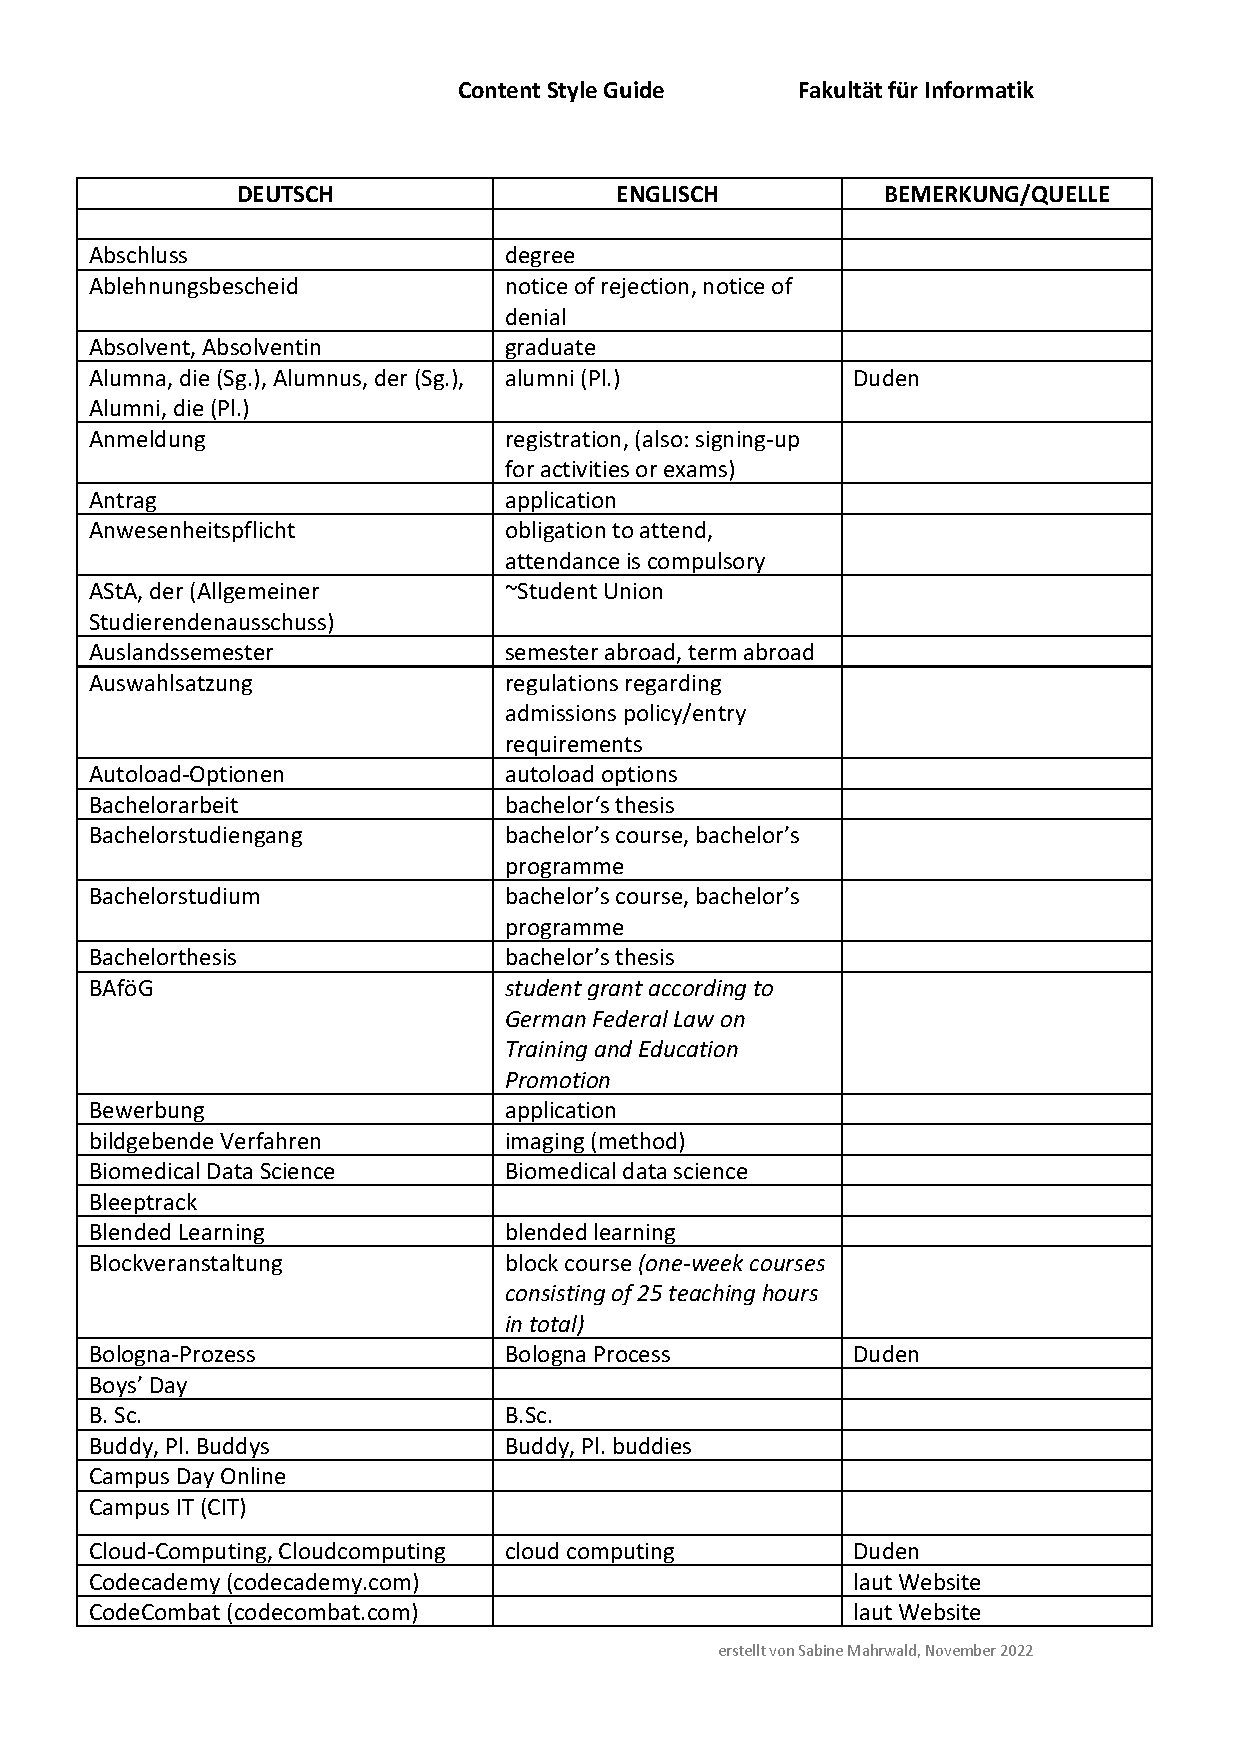
\includepdf[pages=-        % Alle Seiten des Dokumentes einbinden
           ,scale=.8      % Seiten verkleinern, damit sie zum Layout passen
           ,pagecommand={} % Layout des umgebenden Dokumentes belassen
           ]{pdfs/style_guide.pdf}



\end{document}

